% !TeX encoding = UTF-8

%% ------------------------------------------------------------------------
%% Copyright (C) 2021 SJTUG
%% 
%% SJTUBeamer Example Document by SJTUG
%% 
%% SJTUBeamer Example Document is licensed under a
%% Creative Commons Attribution-NonCommercial-ShareAlike 4.0 International License.
%% 
%% You should have received a copy of the license along with this
%% work. If not, see <http://creativecommons.org/licenses/by-nc-sa/4.0/>.
%% -----------------------------------------------------------------------

\documentclass[xcolor=table,dvipsnames,svgnames,aspectratio=169]{ctexbeamer}
% 可以通过 fontset=macnew / fontset=ubuntu / fontset=windows 选项切换字体集

\usepackage{tikz}
\usepackage[normalem]{ulem}
\usetikzlibrary{arrows}
\usepackage{amsmath}
\usepackage{mflogo}
\usepackage{graphicx}
\usepackage{xspace}
\usepackage{amsmath}
\usepackage{unicode-math}
\usepackage{ccicons}
\usepackage{hologo}
\usepackage{colortbl}
\usepackage{shapepar}
\usepackage{hyperxmp}
\usepackage{booktabs}
\usepackage{qrcode}
\usepackage{listings}
\usepackage{tipa}
\usepackage{multicol}
\usepackage{datetime2}
\usepackage{fontawesome5}
\usepackage{hyperref}
\usepackage[backend=biber,style=gb7714-2015]{biblatex}

\addbibresource{biblatex.bib}
\setbeamertemplate{bibliography item}[text]

\graphicspath{{figures/}}

\hypersetup{
  pdfsubject = {PhD-ResearchProposal},
  pdfauthor = {Pedro Hernández Rubio},
  pdfcopyright = {Licensed under CC-BY-SA 4.0. Some rights reserved.},
  pdflicenseurl = {http://creativecommons.org/licenses/by-sa/4.0/},
  unicode            = true,
  psdextra           = true,
  pdfdisplaydoctitle = true
}

\pdfstringdefDisableCommands{
  \let\\\relax
  \let\quad\relax
  \let\hspace\@gobble
}

\renewcommand{\TeX}{\hologo{TeX}}
\renewcommand{\LaTeX}{\hologo{LaTeX}}
\newcommand{\BibTeX}{\hologo{BibTeX}}
\newcommand{\XeTeX}{\hologo{XeTeX}}
\newcommand{\pdfTeX}{\hologo{pdfTeX}}
\newcommand{\LuaTeX}{\hologo{LuaTeX}}
\renewcommand{\CTeX}{C\TeX}
\newcommand{\MiKTeX}{\hologo{MiKTeX}}
\newcommand{\MacTeX}{Mac\hologo{TeX}}
\newcommand{\beamer}{\textsc{beamer}}
\newcommand{\XeLaTeX}{\hologo{Xe}\kern-.13em\LaTeX{}}
\newcommand{\pdfLaTeX}{pdf\LaTeX{}}
\newcommand{\LuaLaTeX}{Lua\LaTeX{}}

\def\TeXLive{\TeX{} Live\xspace}
\let\TL=\TeXLive
\newcommand{\SJTUThesis}{\textsc{SJTUThesis}\xspace}
\newcommand{\SJTUBeamer}{\textsc{SJTUBeamer}\xspace}
\newcommand{\SJTUThesisVersion}{1.0.0rc7}
\newcommand{\SJTUThesisDate}{2020/7/31}

\newcommand\link[1]{\href{#1}{\faLink}}
\newcommand\pkg[1]{\texttt{#1}}

\def\cmd#1{\texttt{\color{DarkBlue}\footnotesize $\backslash$#1}}
\def\env#1{\texttt{\color{DarkBlue}\footnotesize #1}}
\def\cmdxmp#1#2#3{\small{\texttt{\color{DarkBlue}$\backslash$#1}\{#2\}\hspace{1em}\\ $\Rightarrow$\hspace{1em} {#3}\par\vskip1em}}

\lstset{
  language=[LaTeX]TeX,
  basicstyle=\ttfamily\footnotesize,
  tabsize=2,
  keywordstyle=\bfseries\ttfamily\color{cprimary},
  commentstyle=\sl\ttfamily\color[RGB]{100,100,100},
  stringstyle=\ttfamily\color[RGB]{50,50,50},
  extendedchars=true,
  breaklines=true,
}

\lstdefinestyle{style@inline}{
  basicstyle   = \ttfamily,
  keepspaces   = true
}
\lstMakeShortInline[style=style@inline]|

\usetheme[maxplus]{sjtubeamer}
% 使用 maxplus/max/min 切换标题页样式
% 使用 red/blue 切换主色调
% 使用 light/dark 切换亮/暗色模式
% 使用外样式关键词以获得不同的边栏样式
%   miniframes infolines  sidebar* 
%   default    smoothbars split	 
%   shadow     tree       smoothtree
% *siderbar 推荐与 max 一起使用。

% \tikzexternalize[prefix=cache/]
% 如果您需要缓存 tikz 图像,请取消注释上一行,并在编译选项中添加 -shell-escape。

\author{Hugo Vanhille, Pedro Hernández Rubio}
\institute[SEIEE]{Department of Automation}
\date{\the\year 年 \the\month 月}
\subject{ECE6903J - Distributed Machine Learning Systems}
\title{Blockchain-based incentive mechanisms in Federated Learning}
\title[Research project proposal (Group 4)] % 页脚显示标题
{\textbf{Blockchain-based incentive mechanisms in Federated Learning}} % 首页标题

\subtitle{ECE6903J - Distributed Machine Learning Systems (Group 4)}
%\subtitle{Evaluation of blockchain technology in student mobility administration process}

\begin{document}

% 使用节目录
\AtBeginSection[]{
  \begin{frame}
    % \tableofcontents[currentsection]           % 传统节目录             
    \sectionpage                   % 节页
  \end{frame}
}

% 使用小节目录
\AtBeginSubsection[]{                  % 在每小节开始
  \begin{frame}
    % \tableofcontents[currentsection,currentsubsection]             % 传统小节目录             
    \subsectionpage                % 小节页
  \end{frame}
}

\maketitle

\begin{frame}{目录}
\begin{multicols}{2}
  \tableofcontents
  \end{multicols}
\end{frame}

% !TeX encoding = UTF-8
% !TeX root = ../main.tex

%% ------------------------------------------------------------------------
%% Copyright (C) 2021 SJTUG
%% 
%% SJTUBeamer Example Document by SJTUG
%% 
%% SJTUBeamer Example Document is licensed under a
%% Creative Commons Attribution-NonCommercial-ShareAlike 4.0 International License.
%% 
%% You should have received a copy of the license along with this
%% work. If not, see <http://creativecommons.org/licenses/by-nc-sa/4.0/>.
%% -----------------------------------------------------------------------

\section{Background}

\subsection{Motivation}

\begin{frame}{Motivation}
	\begin{block}{Goal}
        Applying ML to systems (blockchain-based models)
      \end{block}
  \begin{itemize}
    \item Research line mainly targeted to \alert{blockchain technology} (its application to systems)
    \item Research group in Department of Automation (PhD supervisors) has been recently working in blockchain-based models applied to \alert{trust management systems}
	\item Specifically, applied to data-aggregation systems in the Internet of Things (IoT) field \alert{crowdsensing}
	\item Could similar approach be applied for \alert{Federated Learning}?
%    \item My PhD thesis could use some of the model simulation techniques (stochastic processes) used in this research paper experimentation
%    \item And of course, it is related to a emerging subfield that could greatly contribute to the development of the Internet of Things (IoT)
  \end{itemize}
\end{frame}

\subsection{Crowdsensing}

\begin{frame}{Crowdsensing: definition}
  \begin{itemize}
  \item \textbf{Crowdsensing:} emerging paradigm of data aggregation\cite{paper1}, having a key role in data-driven applications. Specially used for getting large ammounts of IoT sensing data, by using the individual intelligent sensing devices.
  \item \textbf{Benefit:} improved data collection efficiency and reduced costs effectively\cite{paper2}
  \end{itemize}
  \begin{figure}[h]
        \centering
        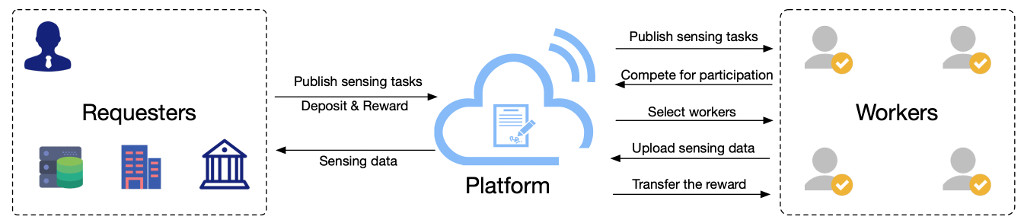
\includegraphics[width=.8\textwidth]{201909-wei-figure1.jpg}
      \end{figure}
\end{frame}

\begin{frame}{Crowdsensing: issues}
  		\begin{enumerate}
   			\item Managed and maintained \alert{centralized platforms} suffer from the single point of failure
   				\begin{itemize}
   					\item \textbf{Proposal: } decentralized architecture (blockchain technology) that lacks a single point of failure, and enhances privacy with asymmetric encryption and digital signature technology
   				\end{itemize}
    		\item Encouraging workers by offering appropiate \alert{incentive mechanisms} (monetary usually) \rightarrow  \underline{auction theory} guarantees benefits for both requesters and workers\cite{paper15} but only provide short-term incentives
    			\begin{itemize}
   					\item \textbf{Proposal:} hybrid incentive mechanism, adopting \underline{mechanism design theory}, considering three factors:
   					\begin{itemize}
   					\item Monetary reward
   					\item Reputation evaluation
   					\item Data quality
   					\end{itemize}
   				\end{itemize}
  		\end{enumerate}
\end{frame}

% !TeX encoding = UTF-8
% !TeX root = ../main.tex

%% ------------------------------------------------------------------------
%% Copyright (C) 2021 SJTUG
%% 
%% SJTUBeamer Example Document by SJTUG
%% 
%% SJTUBeamer Example Document is licensed under a
%% Creative Commons Attribution-NonCommercial-ShareAlike 4.0 International License.
%% 
%% You should have received a copy of the license along with this
%% work. If not, see <http://creativecommons.org/licenses/by-nc-sa/4.0/>.
%% -----------------------------------------------------------------------

\section{Research}

\subsection{Problems}

%\begin{frame}{Research problems}
%\begin{enumerate}
%\item Organizational \textbf{P2P networks} (universities message system): \alert{efficiency?} (messaging time spent and memory space used) $\rightarrow$ \textbf{energy sustainability?}
%\item University network connections (graph theory): \textbf{predicting and recommending partners}: trust? $\rightarrow$ \textbf{links reliability?} \alert{(Machine Learning techniques)}
%\item \textbf{Competitive application calls}: \alert{auction theory (mechanism design)} auditability? $\rightarrow$ \textbf{meritocracy?}
%\end{enumerate}
%\begin{alertblock}{Research studies on practical applications?}
%So far, plenty of theoretical research on blockchain technologies but lack of empirical evidence on real-world practical applications (non-mature and complex technology)
%\end{alertblock}
%\end{frame}

\subsection{The privacy-preserving of Federated Learning}
\begin{frame}{The privacy-preserving of Federated Learning}
    \begin{itemize}
        \item FL provides an attractive structure for decomposing the overall machine learning workflow into the approachable modular units we desire.%(presented in (Kairouz et al.))
        \item FL provides a level of privacy to participating users through data minimization.
    \end{itemize}
    \begin{figure}[h]
        \centering
        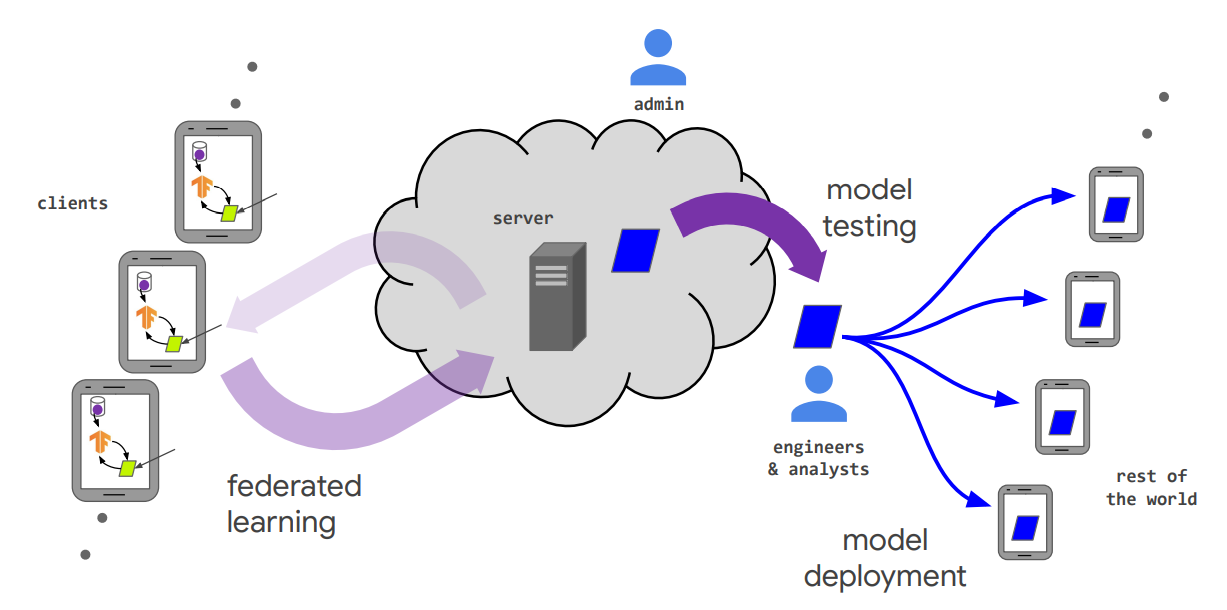
\includegraphics[width=8cm]{structureFL.PNG}
    \end{figure}
\end{frame}

\subsection{The incentive mechanism of Federated Learning}
\begin{frame}{The incentive mechanism of Federated Learning}
  \begin{itemize}
    \item Main types of incentive mechanisms:
          \begin{enumerate}
            \item \alert{Monetary-based}: distributing rewards. %And two subtypes can be considered\cite{paper16}:
            	% \begin{itemize}
            	% \item \alert{price-decision-first} (auction theory) design optimal mechanism benefiting both requesters adn workers
            	% \item \alert{upload-decision-first}: distributing rewards base on the uploaded data (quality)
          		% \end{itemize}
            \item \alert{Reputation-based}: reputation framework for worker selection (algorithms)
          \end{enumerate}
    \item \textbf{Limitations}
    	\begin{enumerate}
            \item Relies on a central platform, vulnerable to target attacks
            \item Single-attribute incentive mechanisms (multifactor incentive needed)
          \end{enumerate}
     %Some previous hybrid incentive mechanisms\cite{paper52} suffer of usability problems because the difficulty of hybrid data management
  \end{itemize}
\end{frame}

%\section{Research}
%
%\subsection{Problems}
%
%\begin{frame}{Blockchain background}
%  \alert{Distributed ledger containing a time-stamped series of immutable blockchains, trustless, decentralized, proof-tampering and full traceability}
%%   \begin{itemize}
%%     \item Research approaches on blockchain-based crowdsensing:
%%           \begin{itemize}
%%             \item Evaluating time consumption and task cost of applying a blockchain-based system\cite{paper33}
%%             \item Blockchain-based crowdsensing quality control model\cite{paper34}
%%             \item Considering privacy issues\cite{paper35}
%%             \item Handling location privacy protection\cite{paper37} (confusion mechanism)
%%           \end{itemize}
%%   \end{itemize}
%    \begin{figure}[h]
%        \centering
%        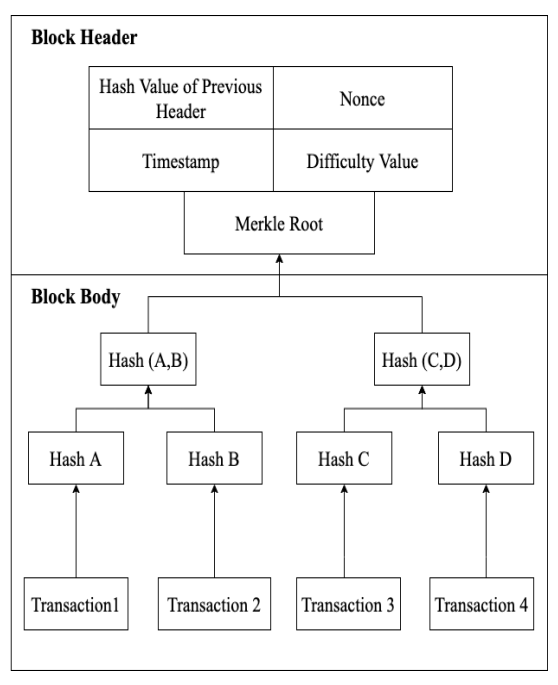
\includegraphics[width=8cm]{topologyBC.PNG}
%    \end{figure}
%\end{frame}
%
%%\begin{frame}{Research problems}
%%\begin{enumerate}
%%\item Organizational \textbf{P2P networks} (universities message system): \alert{efficiency?} (messaging time spent and memory space used) $\rightarrow$ \textbf{energy sustainability?}
%%\item University network connections (graph theory): \textbf{predicting and recommending partners}: trust? $\rightarrow$ \textbf{links reliability?} \alert{(Machine Learning techniques)}
%%\item \textbf{Competitive application calls}: \alert{auction theory (mechanism design)} auditability? $\rightarrow$ \textbf{meritocracy?}
%%\end{enumerate}
%%\begin{alertblock}{Research studies on practical applications?}
%%So far, plenty of theoretical research on blockchain technologies but lack of empirical evidence on real-world practical applications (non-mature and complex technology)
%%\end{alertblock}
%%\end{frame}
%
%\subsection{The privacy-preserving of crowdsensing}
%\begin{frame}{The privacy-preserving of crowdsensing}
%    \begin{itemize}
%        \item FL provides an attractive structure (presented in (Kairouz et al.)) for decomposing the overall machine learning workflow into the approachable modular units we desire.
%        \item FL provides a level of privacy to participating users through data minimization.
%    \end{itemize}
%    \begin{figure}[h]
%        \centering
%        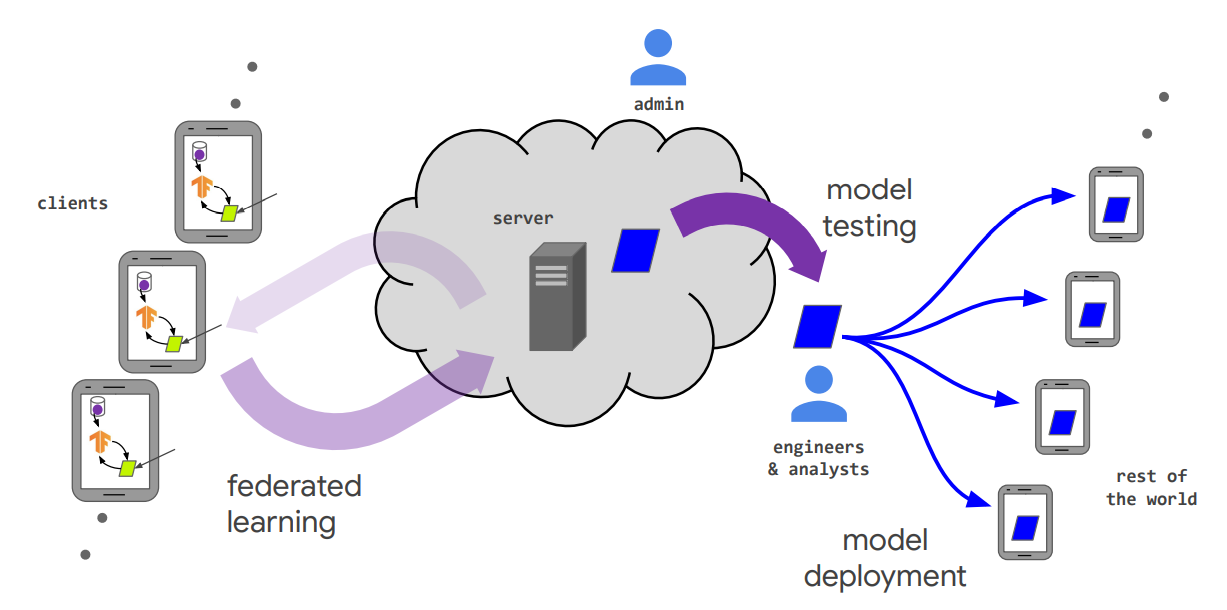
\includegraphics[width=8cm]{structureFL.PNG}
%    \end{figure}
%\end{frame}
%
%\subsection{The incentive mechanism of crowdsensing}
%\begin{frame}{The incentive mechanism of crowdsensing}
%  \begin{itemize}
%    \item Main types of incentive mechanisms:
%          \begin{enumerate}
%            \item \alert{Monetary-based}: distributing rewards. %And two subtypes can be considered\cite{paper16}:
%            	% \begin{itemize}
%            	% \item \alert{price-decision-first} (auction theory) design optimal mechanism benefiting both requesters adn workers
%            	% \item \alert{upload-decision-first}: distributing rewards base on the uploaded data (quality)
%          		% \end{itemize}
%            \item \alert{Reputation-based}: reputation framework for worker selection (algorithms)
%          \end{enumerate}
%    \item \textbf{Limitations}
%    	\begin{enumerate}
%            \item Relies on a central platform, vulnerable to target attacks
%            \item Single-attribute incentive mechanisms (multifactor incentive needed)
%          \end{enumerate}
%     %Some previous hybrid incentive mechanisms\cite{paper52} suffer of usability problems because the difficulty of hybrid data management
%  \end{itemize}
%\end{frame}
%
%%\section{Research}
%%
%%\subsection{Problems}
%%
%%\begin{frame}{Blockchain background}
%%  \alert{Distributed ledger containing a time-stamped series of immutable blockchains, trustless, decentralized, proof-tampering and full traceability}
%%  \begin{itemize}
%%    \item Research approaches on blockchain-based crowdsensing:
%%          \begin{itemize}
%%            \item Evaluating time consumption and task cost of applying a blockchain-based system\cite{paper33}
%%            \item Blockchain-based crowdsensing quality control model\cite{paper34}
%%            \item Considering privacy issues\cite{paper35}
%%            \item Handling location privacy protection\cite{paper37} (confusion mechanism)
%%          \end{itemize}
%%  \end{itemize}
%%\end{frame}
%%
%%%\begin{frame}{Research problems}
%%%\begin{enumerate}
%%%\item Organizational \textbf{P2P networks} (universities message system): \alert{efficiency?} (messaging time spent and memory space used) $\rightarrow$ \textbf{energy sustainability?}
%%%\item University network connections (graph theory): \textbf{predicting and recommending partners}: trust? $\rightarrow$ \textbf{links reliability?} \alert{(Machine Learning techniques)}
%%%\item \textbf{Competitive application calls}: \alert{auction theory (mechanism design)} auditability? $\rightarrow$ \textbf{meritocracy?}
%%%\end{enumerate}
%%%\begin{alertblock}{Research studies on practical applications?}
%%%So far, plenty of theoretical research on blockchain technologies but lack of empirical evidence on real-world practical applications (non-mature and complex technology)
%%%\end{alertblock}
%%%\end{frame}
%%
%%\subsection{The privacy-preserving of crowdsensing}
%%
%%\subsection{The incentive mechanism of crowdsensing}
%%
%%\begin{frame}{The incentive mechanism of crowdsensing}
%%  \begin{itemize}
%%    \item Main types of incentive mechanisms:
%%          \begin{enumerate}
%%            \item \alert{Monetary-based}: distributing rewards. And two subtypes can be considered\cite{paper16}:
%%            	\begin{itemize}
%%            	\item \alert{price-decision-first} (auction theory) design optimal mechanism benefiting both requesters adn workers
%%            	\item \alert{upload-decision-first}: distributing rewards base on the uploaded data (quality)e
%%          		\end{itemize}
%%            \item \alert{Reputation-based}: reputation framework for worker selection (algorithms)
%%          \end{enumerate}
%%    \item \textbf{Limitations}
%%    	\begin{enumerate}
%%            \item Relies on a central platform, vulnerable to target attacks
%%            \item Single-attribute incentive mechanisms (multifactor incentive needed)
%%          \end{enumerate}
%%     Some previous hybrid incentive mechanisms\cite{paper52} suffer of usability problems because the difficulty of hybrid data management
%%  \end{itemize}
%%\end{frame}
%% !TeX encoding = UTF-8
% !TeX root = ../main.tex

%% ------------------------------------------------------------------------
%% Copyright (C) 2021 SJTUG
%% 
%% SJTUBeamer Example Document by SJTUG
%% 
%% SJTUBeamer Example Document is licensed under a
%% Creative Commons Attribution-NonCommercial-ShareAlike 4.0 International License.
%% 
%% You should have received a copy of the license along with this
%% work. If not, see <http://creativecommons.org/licenses/by-nc-sa/4.0/>.
%% -----------------------------------------------------------------------

\section{System architecture}

\subsection{Software application}

\begin{frame}{System architecture}
	\begin{figure}[h]
        \centering
        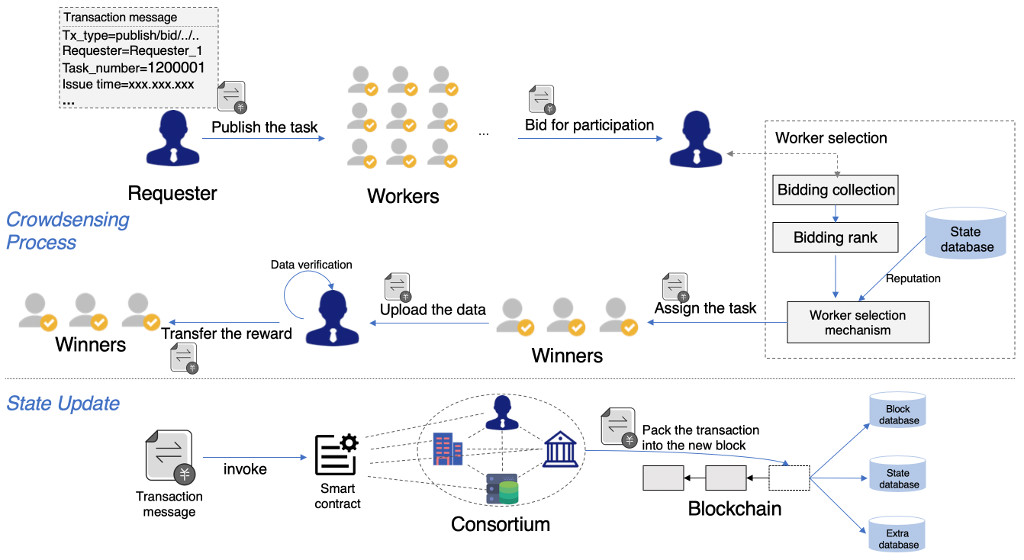
\includegraphics[width=.7\textwidth]{201909-wei-figure2.jpg}
      \end{figure}
\end{frame}

%\begin{frame}{Blockchain application}
%\begin{columns}[T,onlytextwidth]
%    \column{0.7\textwidth}
%	\begin{center}
%		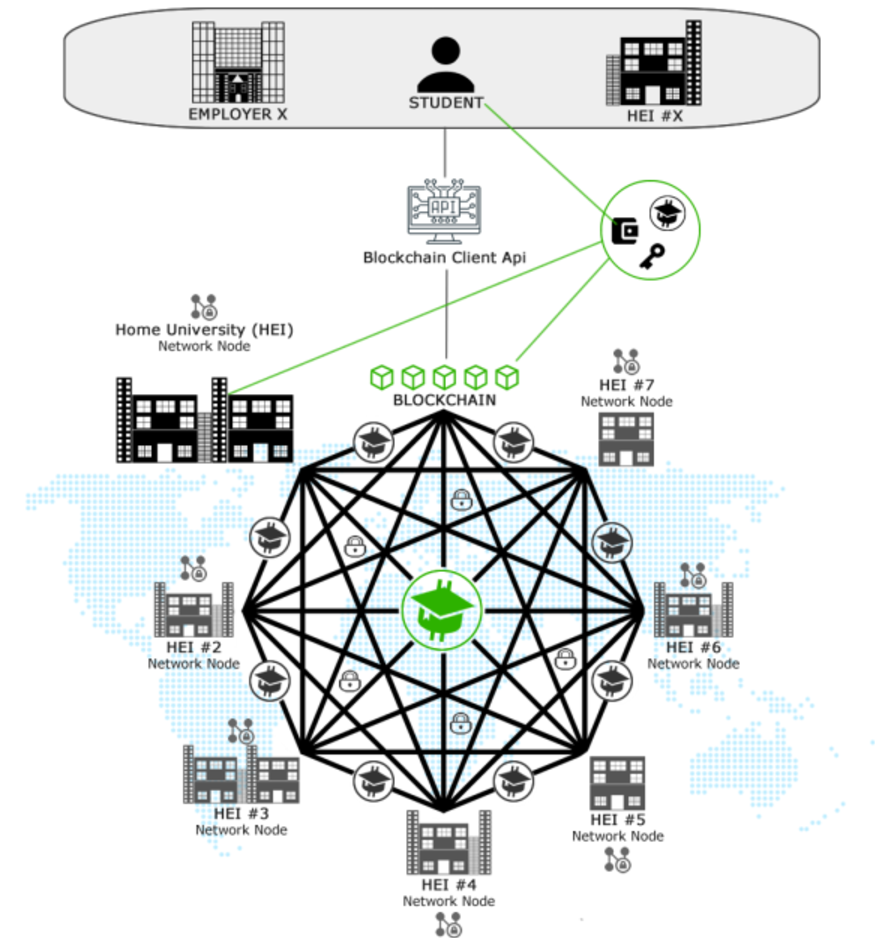
\includegraphics[height=.8\textheight]{eductx.pdf}\hfill
%	\end{center}
%	\column{0.3\textwidth}
%%	\metroset{block=fill}
%      \begin{exampleblock}{Platform}
%        Ethereum
%      \end{exampleblock}
%      \begin{exampleblock}{NF tokens}
%        University credits
%      \end{exampleblock}
%      \begin{exampleblock}{Consensus}
%        Proof-of-stake
%      \end{exampleblock}
%      \begin{exampleblock}{Scope}
%        Public
%      \end{exampleblock}
%      \begin{exampleblock}{Licence}
%        Open source
%      \end{exampleblock}
%\end{columns}
%\end{frame}

%\begin{frame}{Blockchain application}
%  \begin{columns}[c]
%    \begin{column}{.45\textwidth}
%      \begin{itemize}
%        \item Platform
%              \begin{itemize}
%                \item Ethereum
%                \item Hyperledger
%              \end{itemize}
%        \item NF tokens: exchange students
%        \item Consensus: proof-of-stake
%        \item Scope: public
%		\item License: open source
%      \end{itemize}
%    \end{column}
%    \begin{column}{.45\textwidth}
%      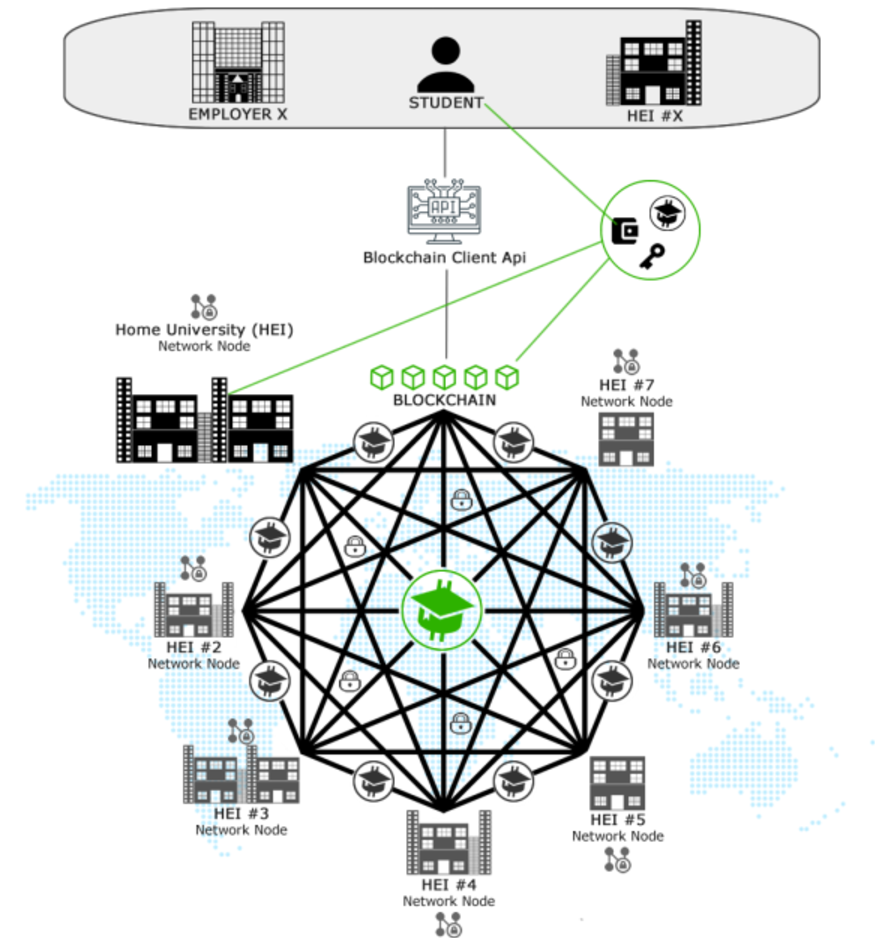
\includegraphics[width=\textwidth]{eductx.pdf}
%    \end{column}
%  \end{columns}
%\end{frame}

\begin{frame}{System flow}
  \begin{itemize}
    \item \textbf{System initialization}: configuration and identity authentication mechanisms
    \item \textbf{Task process}: Specific steps of crowdsensing
          \begin{itemize}
            \item Step 1: \alert{Task publishing} (invoking the smart contract to update the task state)
            \item Step 2: \alert{Worker selection} (workers submit the bidding price and workers select appropiate workers)
            \item Step 3: \alert{Data uploading} (selected workers perform the task and upload data)
            \item Step 4: \alert{Reward assignment and data evaluation} (requester distribute rewards and evaluate data quality)
          \end{itemize}
     \item \textbf{System synchronization}: state update about tasks and workers (validating transactions into new blocks)
  \end{itemize}
\end{frame}

% !TeX encoding = UTF-8
% !TeX root = ../main.tex

%% ------------------------------------------------------------------------
%% Copyright (C) 2021 SJTUG
%% 
%% SJTUBeamer Example Document by SJTUG
%% 
%% SJTUBeamer Example Document is licensed under a
%% Creative Commons Attribution-NonCommercial-ShareAlike 4.0 International License.
%% 
%% You should have received a copy of the license along with this
%% work. If not, see <http://creativecommons.org/licenses/by-nc-sa/4.0/>.
%% -----------------------------------------------------------------------

\section{Related work}

\subsection{Federated Learning}

\begin{frame}
\begin{itemize}

\item \textbf{Advances and Open Problems in Federated Learning\cite{kairouz_advances_2021}}
This paper describes the defining characteristics and challenges of the federated learning setting.It highlights important practical constraints and considerations, and then enumerates a range of valuable research directions. The goals of this paper are to highlight research problems that are of significant theoretical and practical interest, and to encourage research on problems that could have significant real-world impact
\end{itemize}

\begin{itemize}
\item \textbf{Generative models for effective ML in  private, decentralized datasets\cite{augenstein_generative_2020}}

This document focuses on three main topics : 
\begin{itemize}
\item Identifying key challenges in implementing end-to-end workflows with non-inspectable data
\item Proposing a methodology that allows ‘auxiliary’ generative models to resolve these challenges
\item Demonstrating how privacy preserving federated generative models can be trained to high enough fidelity to discover introduced data errors matching those encountered in real world scenarios
\end{itemize}
\end{itemize}
\end{frame}

\subsection{Blockchain-based Federated Learning}

\begin{frame}
\begin{itemize}
\item \textbf{Blockchain-based Federated Learning: A Comprehensive Survey\cite{wang_blockchain-based_2021}}

This paper conducts a comprehensive survey of the literature on blockchained FL (BCFL). First, it investigates how blockchain can be applied to federal learning from the perspective of system composition. Then, it analyzes the concrete functions of BCFL from the perspective of mechanism design and illustrate what problems blockchain addresses specifically for FL. Finally, it discusses some challenges and future research directions.

\item \textbf{Federated Learning Meets Blockchain in Edge Computing: Opportunities and Challenges\cite{nguyen_federated_2021}}

This article presents an overview of the fundamental concepts and explores the opportunities of FL chain in mobile-edge computing networks in relation with his main issues in FL chain design such as communication cost, resource allocation, incentive mechanism, security and privacy protection. The key solutions and the lessons learned along with the outlooks are also discussed. Then, it investigates the applications of FL chain in popular Mobile-edge computing domains.
\end{itemize}

\end{frame}

\subsection{Hybrid incentives for contributions}

\begin{frame}
\begin{itemize}
\item \textbf{Record and Reward Federated Learning Contributions with Blockchain\cite{martinez_record_2019}}

When contributing with local data to Federated Learning systems, this paper deals with the issues of data security and paying workers with appropriate rewards based on the data quality of contributions. A Blockchain design based on validation error based metric (in order to qualify gradient uploads for rewarding) is presented. Limitations are found regarding both inefficiency and inaccuracy in rewarding participant contributions and lack of scalability of data.

\item \textbf{Transparent Contribution Evaluation for Secure Federated Learning on Blockchain\cite{ma_transparent_2021}}

This article focus on privacy issues because of blockchain data being public to all contributors. Proposed solutions:
\begin{itemize}
\item Blockchain-based privacy-preserved FL with secure aggregation (mask updates) in order to protect data owner's privacy during training.
\item A group-based Shapley value-based computation framework with secure aggregation (contribution evaluation protocol)
\end{itemize}
\end{itemize}

\end{frame}

\subsection{Mechanism designs: theory}

\begin{frame}
\begin{itemize}
\item \textbf{Blockchain-Enabled Federated Learning With Mechanism Design\cite{toyoda_blockchain-enabled_2020}}

This work researchs theoretically about rewarding impacts contributor's behavior and defining appropriate qualitative rewards to the parcipants. In order to improve competition for model updating process, Mechanism Design theory is analyzed, specifically by leveraging contest and auction theory, in order to increase contributors' motivation and to maximize rewards. Some mathematical conditions regarding protocol design are found to be necessary for a successful application of contest theory in this scenario.
Summing up, incentive-aware Federated Learning (crowsourcing) with Mechanism Design is a promising research theory and practical experimentation is needed.

\end{itemize}

\end{frame}

% !TeX encoding = UTF-8
% !TeX root = ../main.tex

%% ------------------------------------------------------------------------
%% Copyright (C) 2021 SJTUG
%% 
%% SJTUBeamer Example Document by SJTUG
%% 
%% SJTUBeamer Example Document is licensed under a
%% Creative Commons Attribution-NonCommercial-ShareAlike 4.0 International License.
%% 
%% You should have received a copy of the license along with this
%% work. If not, see <http://creativecommons.org/licenses/by-nc-sa/4.0/>.
%% -----------------------------------------------------------------------

\section{Planned solutions}

\subsection{ML for system}

\begin{frame}{Mechanism design: multifactor issue (static)}
\begin{multicols}{2}
  \begin{itemize}
    \item Based on \textbf{static} parameters:
          \begin{enumerate}
            \item \alert{Workers' bidding}
            \item \alert{Reputation}
            \item \alert{Recent data quality estimation}
          \end{enumerate}
    \item Analytic Hierarchy Process (AHP)
    	\begin{enumerate}
            \item \alert{Objective level}: winning workers
            \item \alert{Criteria level}: parameters criteria
            \item \alert{Alternative level}: workers available
          \end{enumerate}
    \end{itemize}
\end{multicols}
    \begin{exampleblock}{Multifactor worker evaluation approach (example)}
    	\begin{equation*}
      	\theta_{i}=\omega_{1} B_{i}+\omega_{2} R_{i}+\omega_{3} Q_{i} \quad\quad \text { where } \omega_{i} \geq 0 \text { and } \sum_{\omega_{i}=1}^{3} \omega_{i}=1	
    	\end{equation*}
  \end{exampleblock}
  \begin{block}{Approach: ML for system}
  	Dynamic evaluation parameters for the incentive model (ML techniques)
  \end{block}
\end{frame}

%\begin{frame}{Mechanism design: issues}
%  		\begin{enumerate}
%   			\item \textbf{How to select appropriate workers?}
%   				\begin{itemize}
%   					\item \textbf{Proposal: } decentralized architecture (blockchain technology) that lacks a single point of failure, and enhances privacy with asymmetric encryption and digital signature technology
%   				\end{itemize}
%    		\item \textbf{How to distribute the rewards to the workers?}
%  		\end{enumerate}
%  		With the help of \alert{mechanism design theory}\cite{article56} two important properties for the incentive mechanism are guaranteed:
%  		\begin{itemize}
%   					\item \textbf{Incentive quality (IC):} the truthful submission of sensing  cost is the worker's optimal bidding strategy
%   					\item \textbf{Individual rationality (IR):} the reward must compensate for the worker's cost (non-negative)
%   		\end{itemize}
%\end{frame}

\subsection{Bonus: System for ML}

\begin{frame}{System efficiency: consensus protocol}
\alert{Blockchain-based Federated Learning (FL)}
  \begin{itemize}
    \item Potential bottlenecks:
    	\begin{enumerate}
            \item Transaction throughput
            \item Lack of scalability of data
          \end{enumerate}
    \end{itemize}

  \begin{block}{Approach: System for ML}
  	Optimization of consensus protocol in FL (better performance)
  \end{block}
\end{frame}

%%+% !TeX encoding = UTF-8
% !TeX root = ../main.tex

%% ------------------------------------------------------------------------
%% Copyright (C) 2021 SJTUG
%% 
%% SJTUBeamer Example Document by SJTUG
%% 
%% SJTUBeamer Example Document is licensed under a
%% Creative Commons Attribution-NonCommercial-ShareAlike 4.0 International License.
%% 
%% You should have received a copy of the license along with this
%% work. If not, see <http://creativecommons.org/licenses/by-nc-sa/4.0/>.
%% -----------------------------------------------------------------------

\section{Conclusions}

\subsection{Application}

\begin{frame}{Results}
	A consortium blockchain-based incentive model for crowdsensing system is
proposed
  \begin{itemize}
  \item \textbf{Benefits of consortium blockchain technology:} 
  	\begin{itemize}
  		\item resistant to the single point of failure (system security)
  		\item cooperative management (by requesters) reduces cost and enhances the flexibility of the system (selection criteria)
  	\end{itemize}
  \item \textbf{Benefits of hybrid incentive mechanism:}
  	\begin{itemize}
  		\item encourages workers to contribute valuable data (and penalizes malicious ones)
  		\item ensures favorables short-term and long-term incentives for workers
  	\end{itemize}
  \end{itemize}
\end{frame}


\subsection{Limitations}

\begin{frame}{Limitations}
	Further research:
  \begin{enumerate}
  \item Dynamic situation where evaluations attributes are changing
  \item Optimization of consensus protocol (better performance)
  \item Further protection of worker privacy
  \end{enumerate}
  \begin{block}{Possible solutions}
  Application of ML techniques to blockchain-based system
  \end{block}
\end{frame}

\subsection{Further research}
% !TeX encoding = UTF-8
% !TeX root = ../main.tex

%% ------------------------------------------------------------------------
%% Copyright (C) 2021 SJTUG
%% 
%% SJTUBeamer Example Document by SJTUG
%% 
%% SJTUBeamer Example Document is licensed under a
%% Creative Commons Attribution-NonCommercial-ShareAlike 4.0 International License.
%% 
%% You should have received a copy of the license along with this
%% work. If not, see <http://creativecommons.org/licenses/by-nc-sa/4.0/>.
%% -----------------------------------------------------------------------

\section{Goals}

\subsection{Task assignment}

\begin{frame}{Task assignment}
	Collaboration through online tools:
  \begin{itemize}
  	\item \alert{GitHub} Documentation repository \url{https://github.com/pedroherub/dmls-project}
  	\item \alert{Zotero} References (group)  \url{https://www.zotero.org/groups/4822089/dmls-project}
  \end{itemize}
  Tasks distribution:
  \begin{itemize}
  	\item \textbf{Hugo Vanhille:} Research focus on blockchain-based Federated Learning \& Zotero group management
  	\item \textbf{Pedro Hernández:} Research focus on blockchain-based incentive models and mechanism design \& Latex editing
  \end{itemize}
\end{frame}

\subsection{Goals}

\begin{frame}{Bottom-line outcome}
\begin{itemize}
\item State of the art of blockchain-based Federated Learning as \alert{trust management systems}
\item Determine the characteristics required to have a good trust FL system:
	\begin{itemize}
		\item Security
		\item Efficiency
		\item Incentives
	\end{itemize}
\item Sum up the actual issues of trust FL systems and suggest approaches that could solve these limits
\end{itemize}

\end{frame}

\subsection{Bonuses}

\begin{frame}{PhD research proposal}
\begin{block}{In search of research ideas}
  Blockchain-based Federated Learning: trusted management systems
\end{block}
PhD supervisors:
  \begin{itemize}
  	\item \textbf{Long Chengnian} SEIEE, Department of Automation \url{https://automation.sjtu.edu.cn/Chengnian}
  	\item \textbf{Jing Wu} SEIEE, Department of Automation \url{https://automation.sjtu.edu.cn/Jing}
  \end{itemize}
  \begin{alertblock}{Research lines}
    Trusted AI, AIoT, Blockchain, Cyber-Physical Systems
\end{alertblock}
\end{frame}

\begin{frame}{Conferences}
	Potential paper submission for the following conferences:
  \begin{itemize}
  	\item \textbf{ICBCT 2023:} 5th International Conference on Blockchain Technology (organized by Shanghai Jiao Tong University) \url{https://icbct.org/} [March 2023]
  	\item \textbf{MLSys 2024:} 7th Conference on Machine Learning and Systems  \url{https://mlsys.org/} [June 2024]
  \end{itemize}
\end{frame}
% !TeX encoding = UTF-8
% !TeX root = ../main.tex

%% ------------------------------------------------------------------------
%% Copyright (C) 2021 SJTUG
%% 
%% SJTUBeamer Example Document by SJTUG
%% 
%% SJTUBeamer Example Document is licensed under a
%% Creative Commons Attribution-NonCommercial-ShareAlike 4.0 International License.
%% 
%% You should have received a copy of the license along with this
%% work. If not, see <http://creativecommons.org/licenses/by-nc-sa/4.0/>.
%% -----------------------------------------------------------------------

\section{Schedule}

\subsection{Timeline}

\begin{frame}{Tentative schedule}
%  \begin{enumerate}
%  \item \textbf{Redefining research proposal:} until June 2022
%  \item \textbf{Publishing 3 papers:} approximately one each academic year
%  \end{enumerate}
  \begin{figure}[h]
        \centering
        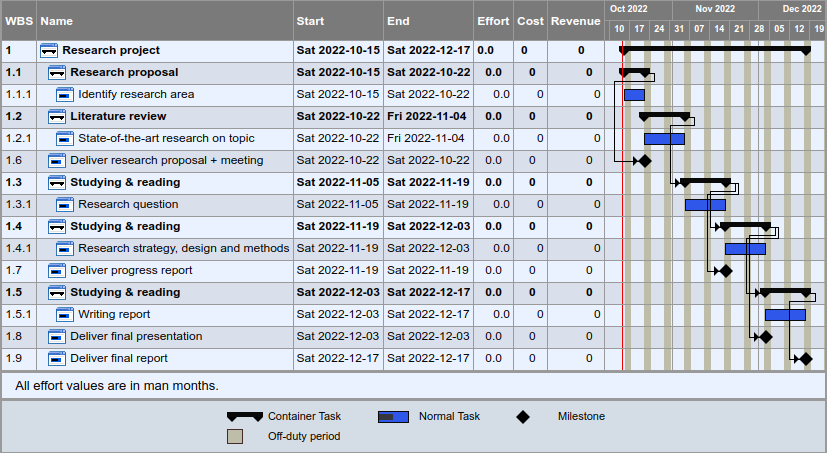
\includegraphics[width=.7\textwidth]{gantt.png}
      \end{figure}
\end{frame}

\appendix

\begin{frame}[allowframebreaks]
  \frametitle{参考文献}
  \printbibliography
\end{frame}

\makebottom

\end{document}
